\section{横向速度变化}
\label{sec:3.7}

对于进行解释的地质家来说,横向速度变化就是使地震剖面中产生了强烈畸变。其实,
畸变比它看上去的样子还要糟。地球物理学家则面临着挑战,试图以定量方式去处理速度横
向变化问题。首先是,如何才能可靠地估计横向速度变化的大小?然后是,我们敢将这些估
计用于重处理数据吗?

我们从倾角和炮检距的研究中已经得出了掌握它们的直接处理办法了,即使在二者同时
存在时,也能应付得了。遗憾的是,显著的横向速度变化导致了显著的混乱,我们必须想办法克
服的就是这种混乱。强烈的横向速度变化掩盖了北美Prudhoe海湾的最大油田。幸好,我们有
许多易于理解的理想化例子,任何“终极的”理论都不得不把这些例子作为极限情形来解释。

让我们回顾一下。如把平方根展开,而且如果我们接受精确度受倾斜角度影响的通常限
制,那么双平方根方程大掘是可以起作用的。双平方根方程的问题是,它仅只告诉我们一旦
速度已知时应如何偏移与叠加。确定速度分布$v(x,z)$的Kjartansson方法要假设有直射线、
没有倾角、而且是一个平反射面才行。另一方面,同叠前局部偏移一起进行的叠加,允许有任
何散射体几何形态,但是仅在不存在横向速度变化的假设下才能确定速度。很清楚,这
里还有许多问题有待解决。我们将从易于理解的特殊情形开始讨论,虽说是特殊情形,但却
能非常深入问题的本质。


\subsection{替代速度---使海水层冻结起来}
\label{sec:3.7.1}

有时运气好,可以知道速度。也许你知道速度是因为你正在处理合成地震资料;也许你
知道它是因为你已经钻了三百个浅孔;或许你能够作出很好的估计是因为你手上有已经知道
海水层深度的剖面资料,所以你才愿意去猜测沉积地层的速度。实际上,速度问题往往是一
种表层中存在的问题。或许你的地震电缆正巧从红海内不常见的灰岩礁上拖曳而过,因而你
可能知道速度。

假定速度已知并已知近地表商处有癀向变化,这时你应考虑采用关于替代速度(repla
cement velocity)的思想。例如,假如你能叫红海的海水冻结起来,恰好使它硬到足以使一
冰层速度与灰岩礁速度相等为止,那样就会消除深层反射的不必要的复杂性。当然,你不可
能真使红海冻结,但是你可以将资料重新处理,试图去摹拟如果你能作到使它冻结时就会记
录到的地震资料。

首先,把数据资料向下延拓至速度横向变化带以下的某个基准面,然后经过均匀的替代
介质将它向上延拓返回至地面。

尽管原则上是可以将双平方根方程应用于这项目的,可是实际利用它太费时间,因而不
大现实。最好的办法是研究出一种把上行与下行两种运算结合在一起的方法。既然这域种运
算大部分是彼此反向的,则无论怎样处理资料都应该只是一种差函数。例如,下列方程:
\begin{equation}
\frac{\partial P}{\partial z}=i\omega[\frac{1}{v(s)}+\frac{1}{v(g)}-\frac{2}{v_{avg}}]P
\label{eq:ex3.7.1}
\end{equation}
就是将向下延拓同向上延拓结合起来了,因而在各项速度近乎相同时,只不过使波场尸有很
小变化。方程\ref{eq:ex3.7.1}基本上是一种时移方程。有一种以静校正而著称的生产性处理方
法,“静”这个词意味着时不变,亦即时移的大小不随时间而变。当适宜的校正仅仅是静态
时移时,地层模型就只在近地面处才有横向速度变化,情形往往就是如此。因为速度$v(s)$
与$v(g)$可以是深度$z$的任何函数,所以方程\ref{eq:ex3.7.1}也有能力作时变的时移。由于正规采
用的是较大的炮检距,所张角度属于广角,因而有希望把方程\ref{eq:ex3.7.1}推广到广角情形。
在Lynn(1979年)的论文内即有这类推广。Lynn还指出:如何才能写出偏微分方程去描述
横向速度变化对叠加速度的影响。BerryhilK(1979)阐述了采用Kirchhoff方法处理不规则基准面的问题。

在实际应用中,对横向速度变化进行估计的问题通常比偏移时应用这些速度要麻烦得
多。根据大量观测,包括高程测量、由炮井底部至地表的旅行时间测定、以及反射地震记录互
相关函数的计算等,估计出静态时移。Wiggins等人(1976
)曾提出过一种根据相关观测确定静态时移的方法。

在较深层也有速度横向变化的地方,时移变成与时间有关,这种情形称作动态时移问
题。为计算动态时移,得假设倾角为零。通过一假想的具有横向可变速度的模型作射线追
踪;再通过一具有横向恒定速度的参考模型作射线追踪。这两种模型的旅行时间之差就定义
了动态时移,见图\ref{fig:vdmo/dent}该处的横向变化涉及范围还很深,所以问题看上去更像是一个偏
移问题。图\ref{fig:vdmo/reveal}是Digicon公司采用一种称作REVEAL的处理方法所得结果,不过他们没
有透露究竟采用的是时移方法还是波动方程方法。

\begin{figure}[H]
\centering
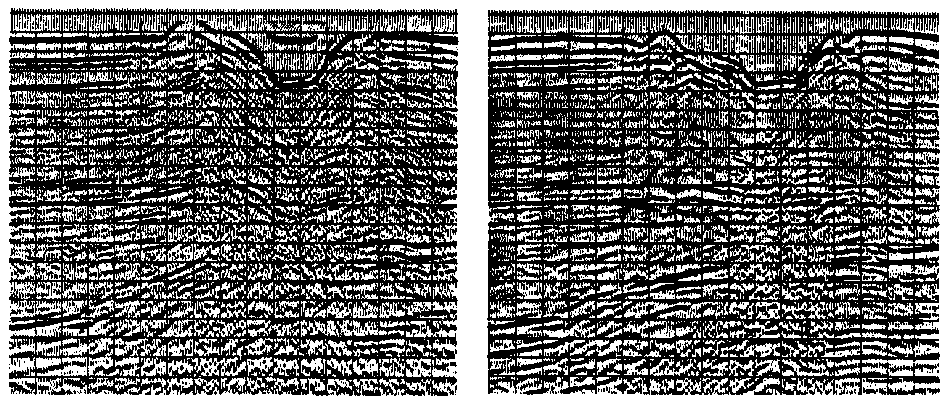
\includegraphics[width=0.65\textwidth]{vdmo/dent}
\caption[dent]{菲律宾地区的资料(左图),经过动态时移校正之后的结果(右图)(据 Dent,1983)}
\label{fig:vdmo/dent}
\end{figure}

\begin{figure}[H]
\centering
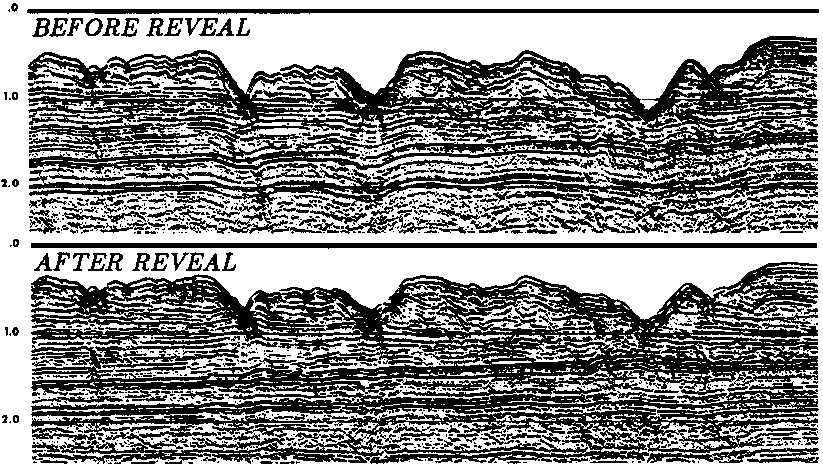
\includegraphics[width=0.65\textwidth]{vdmo/reveal}
\caption[reveal]{采用替代速度进行处理的例子。
可以看出,较深的地层现已较平缓且更连续(Digicon公司提供)}
\label{fig:vdmo/reveal}
\end{figure}

\subsection{双曲线顶点的横向移动}
\label{sec:3.7.2}

图\ref{fig:vdmo/lady}所示是一个点散射体,位于呈三十度倾斜的低速楔形层之下的高速层内,这是许
多横向速度变化问题的一种典型情形。地表上的到达时间将是粗略呈双曲线形,但具有某种畸
变,因为在分界面上出现有速度跳跃变化。时距曲线的极小(即双曲线的顶点)业已偏离它
的通常位置,不是正在该点射散体之上方。可以看出:
\begin{enumerate}
  \item 在极小时间时,射线垂直向上出射;
  \item 极小时间位于该点散射体所在的高速一侧;
  \item 极小时间偏离该散射点的位移,随炮检距之增大而增加。
\end{enumerate}
时距曲线大体呈双曲线形,但是左侧的渐近线给出左侧介质的速度,而右侧的渐近线则给出
右侧介质的速度。

\begin{figure}[H]
\centering
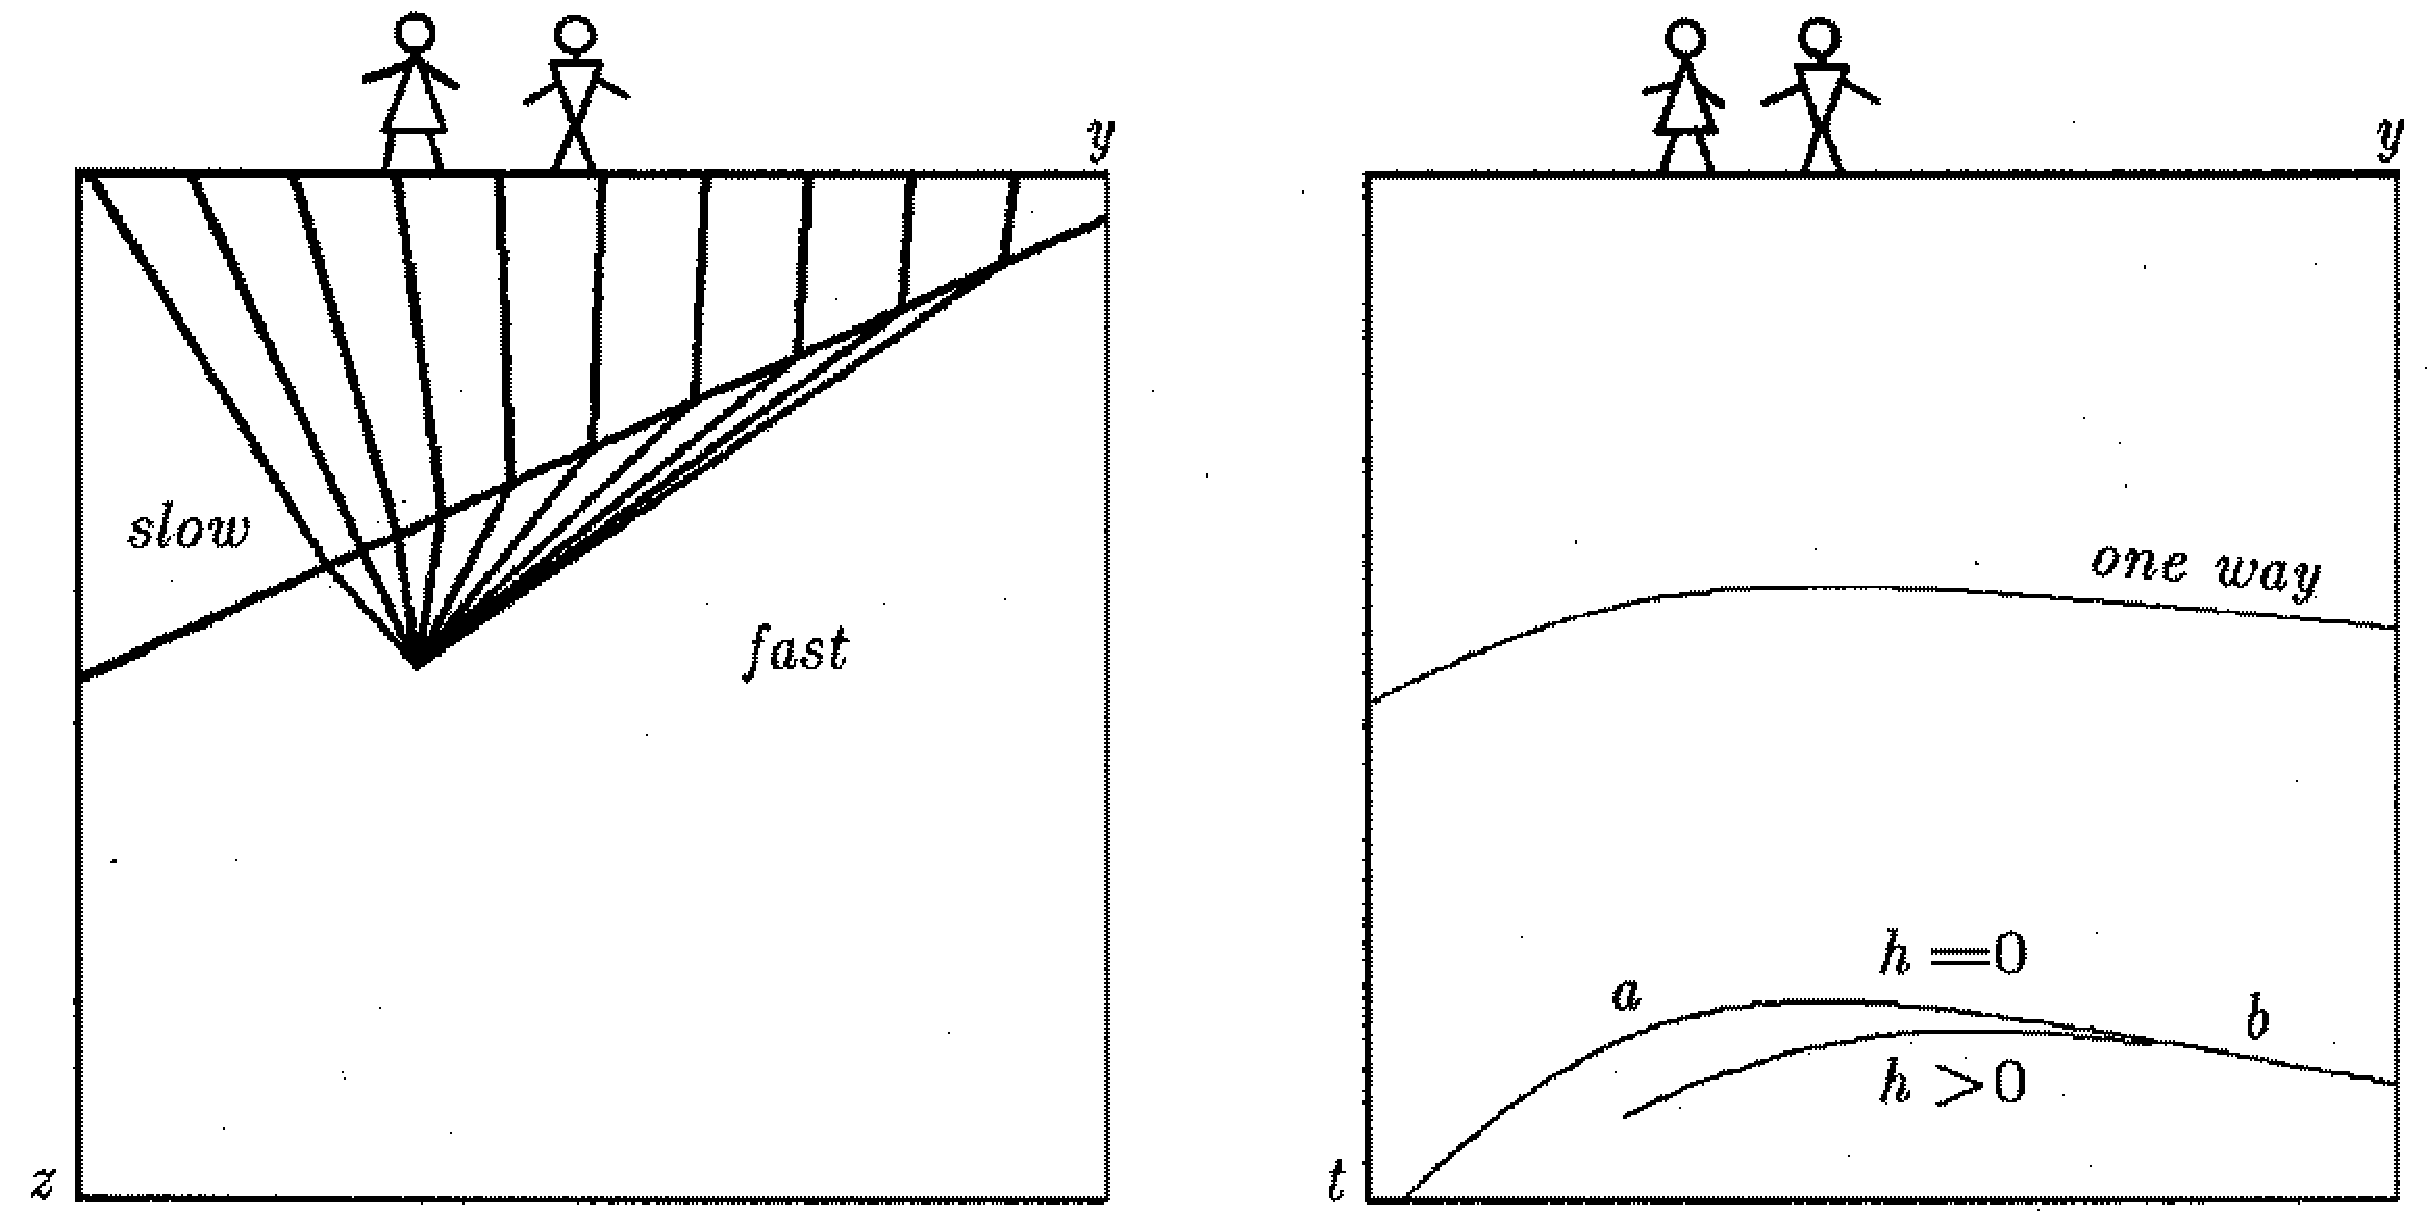
\includegraphics[width=0.65\textwidth]{vdmo/lady}
\caption[lady]{位于速度楔形层之下的散射点的出射线(左图),时距曲线(右图)。
图中,a点处的斜率是b点处斜率之负值。a与b之间的中点位于$h>0$时的曲线之顶部}
\label{fig:vdmo/lady}
\end{figure}

设自散射点至地面$x$点的旅行时间记为$T(x)$,这时对共炮检距剖面来说,旅行时间$t(y)$
就是
\begin{equation*}
t(y)=T(y+h)+T(y-h)
\end{equation*}
为求出最早到达的初至,令$dt/dy=0$,由此可证明图\ref{fig:vdmo/lady}中的$a$点上的斜率应是$b$点上斜率
之负值。这点表明了为什么双曲线顶部偏离散射体的位移是随炮检距而增大的\footnote{
必须同时还考虑到双曲线的不对称性质,才能得此结论。---译者
}。

横向速度变化使双曲线丧失了对称性,从计算上说,这就是透镜项使双曲线发生了歪
斜,引起了它的顶点作横向移动。

\subsection{“幽灵”绕射}
\label{sec:3.7.3}

横向速度变化的第二个例子
是图\ref{fig:vdmo/westdepthmig},该图也是取自Kja-
rtansson的博士论文。图中所示物理模型是由代表反射面之断续
线段所分开的三个具有恒定速度的楔形层,该模型的底边也代表
一个反射面。图\ref{fig:vdmo/westdepthmig}中的波场
利用爆炸反射面计算方法作出, Kjartansson把该种计算方法看
作是零炮检距剖面的合理近似。注意,在速度为4公里/秒的楔形
层尖端的下方,在底部水平反射面上有一个小绕射。因为这样一
种绕射与可辨认出的平坦反射面毫无关系,所以给它取名为“幽
灵”绕射(Phantom diffraction)。幽灵绕射本容易识别,
但是它们确实会出现。实际上, \ref{sec:3.1}节中所述的“亮点”大概就
是幽灵绕射;有人曾报导过,幽灵绕射为勘探小型的高速灰岩礁
提供了一种工具。

\begin{figure}[H]
\centering
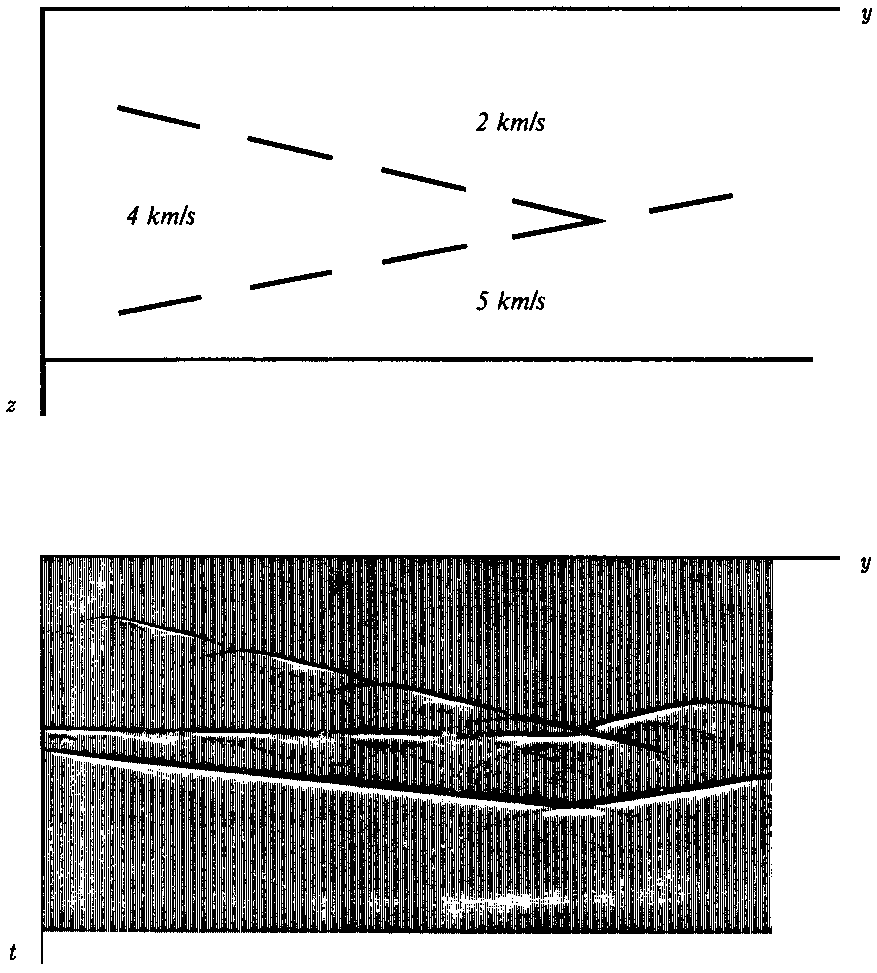
\includegraphics[width=0.65\textwidth]{vdmo/westdepthmig}
\caption[westdepthmig]{上图的模型取自西方地球物理公司的深度偏移
方法小册子。该模型并非有物理意义的模型,因为分界面都是呈片段状;不过
,这类片段却可成为研究横向移位的很好案例。下图为合成资料(据Kjartansson),
幽灵绕射正位于楔形层尖端之下方,出现在到达时间最晚之处。}
\label{fig:vdmo/westdepthmig}
\end{figure}


\subsection{波阵面愈合}
\label{sec:3.7.4}

图\ref{fig:vdmo/heal}是射线发生弯曲的另一种例子,左边第一个画面表
示平面波刚好在因薄透镜项影响而已畸变为波状起伏形之后的情形。此后一个画面是薄透镜
项的影响消失了,以后的各画面所示是不断増大的绕射影响。

\begin{figure}[H]
\centering
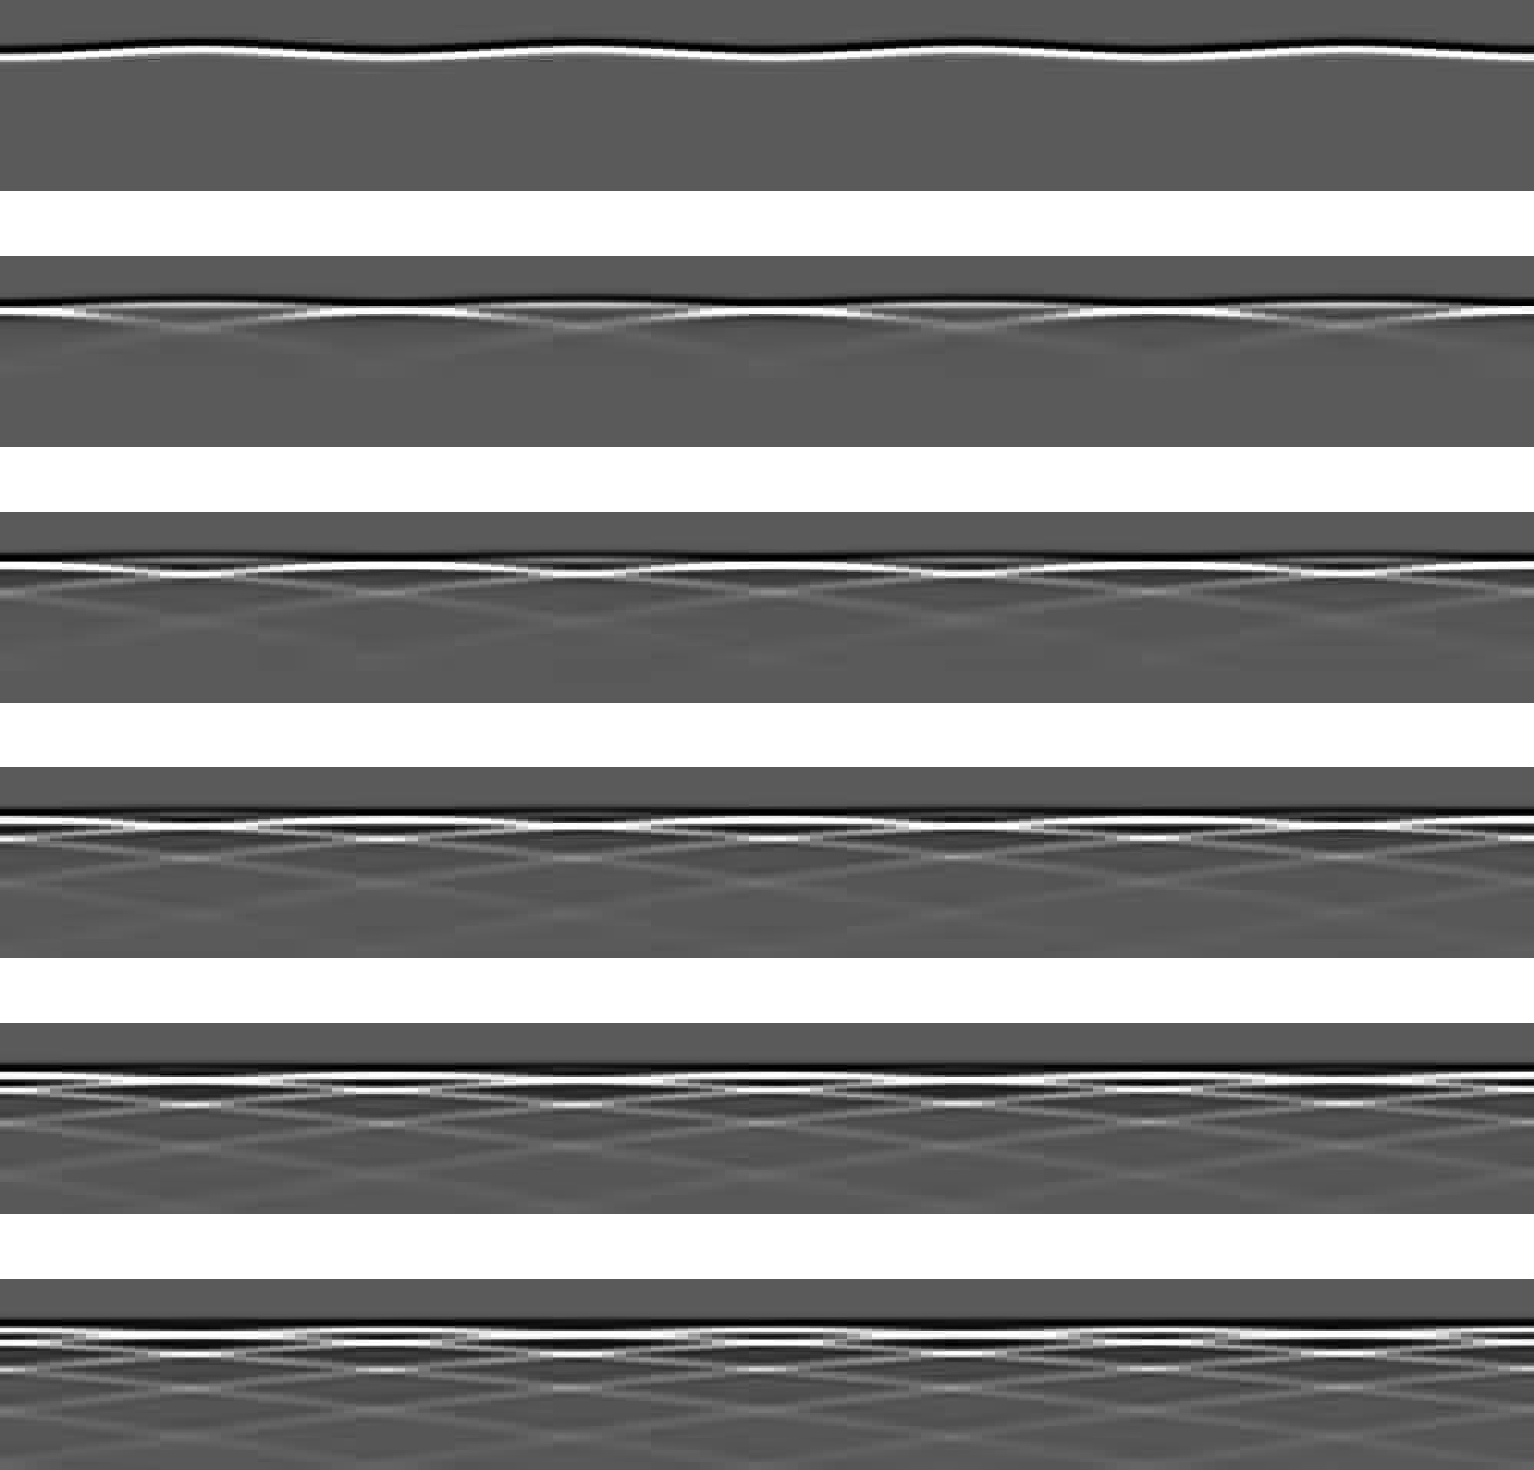
\includegraphics[width=0.65\textwidth]{vdmo/heal}
\caption[heal]{左侧第一个画面所示是刚好因薄透镜项影响而畸变为波状之后的平面波
。在此之后,薄透镜项的作用消失。以后的相继画面所示是绕射影响不断增大。注意波束拉长
和初至愈合的现象(取自《地球物理数据处理基础》一书,页213)}
\label{fig:vdmo/heal}
\end{figure}

\subsection{断层面反射}
\label{sec:3.7.5}

通过地层内一个垂直断层时,速度变化将是水平坐标的一个简单阶跃函数。因为反射系
数和透射系数与角度有关,传播通过这样一种断层的射线会经受振幅变化。由于有共同的近
于垂直的射线,只要存在很小的速度差异就能产生很强的内部反射。根据这个道理,陡断层
应当是畸变得更多,从而断层在小炮
检距剖面上就比大炮检距剖面或叠加更容易辨别出来。

在$(y,t)$空间内观察时,这种现象就有点更为混乱。图\ref{fig:vdmo/veljump}系由Kjart
ansson计算出,他曾在一次测验中将该图作为考试题目。请你研究
一下这个图并回答说明中提出的那些问题。这里提示一下:超过临界角的
反射射线要经历相移的变化,这会把一个脉冲变成双脉冲,很容易误认为
是有两种射线路程。

\begin{figure}[H]
\centering
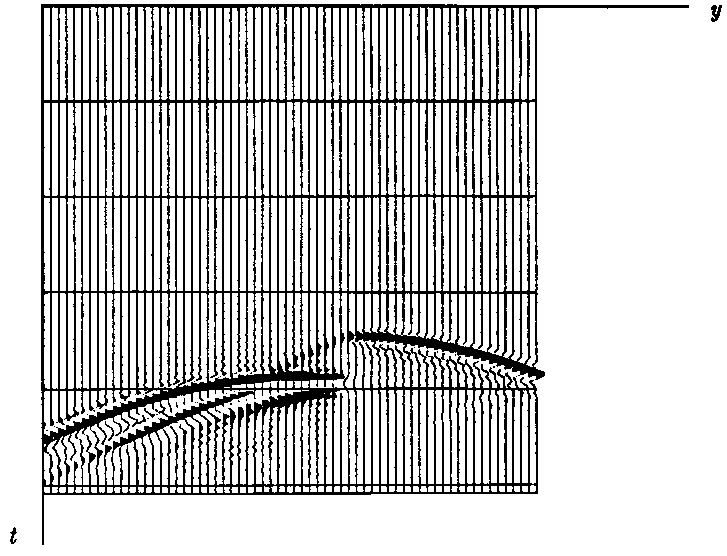
\includegraphics[width=0.65\textwidth]{vdmo/veljump}
\caption[veljump]{包含有一散射点并在通过垂直接触面时存在速度
跃变$v_1/v_2=1.2$的地层模型,根据爆炸反射面概念计算出的合成
时间剖面(据Kjartansson)}
\label{fig:vdmo/veljump}
\end{figure}


图\ref{fig:vdmo/veljump}展现的剖面形态说明爆炸反射面模型无法产生零炮检距剖面
上能见到的所有射线。爆炸反射面模型产生两种类型射线:直接抵达地面
的射线和到达地面以前由断层面反射的射线。零炮检距剖面则有三类射线:
两种射线路程与前述相同,但有双倍旅行时间,一次是上行,一次是下行;
另外就是图\ref{fig:vdmo/veljump}中没出现的射线,
即在一个路程中遇到断层面而在另一个路程中则遇不到断层面。

当反射体只是一个点时,要作横向可变介质中的共炮检距剖面有一个简单办法,就是把
点上记录到的爆炸反射面地震记录直接就同点上所记录到的爆炸反射面地震记录按
时间进行褶积。褶积使旅行时间增大,甚至产生了非爆炸反射面的射线。很糟糕的是,这种
技术对于比一个简单的反射点更复杂的反射面糢型却并非有效。




% \subsection{习题}
% \label{sec:3.6.6}

% \begin{enumerate}
% \item 试述Hale的倾角时差校正处理中Jacobi函数行列式的影响。

% \end{enumerate}
